\section{Sequence diagrams}\label{app:seq}
All diagrams are simplified in the sense that they do not show every atomic operation and that they show only validation and error handling when it is relevant and essential to the understanding of the sequences. They are simplified to improve the overall orderliness and comprehensibility of the diagrams.
\begin{figure}[hb]
  \centering
  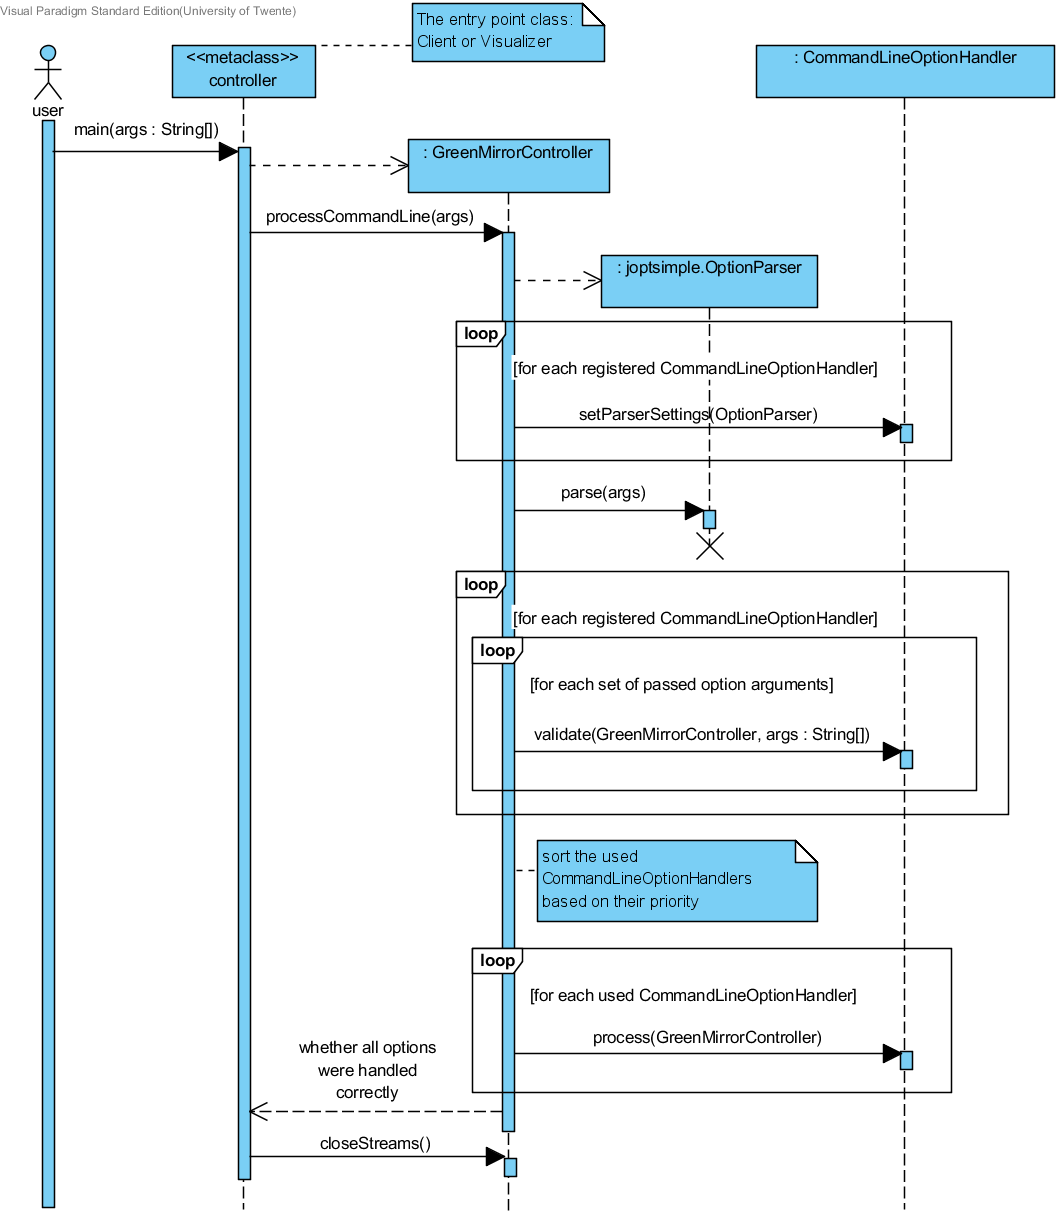
\includegraphics[width=0.96\textwidth]{diagrams/SD_generalstartup}
  \caption{simplified sequence diagram of the general start-up. There is a slight difference on the server side: if the options are all handled correctly, the controller doesn't close the streams, but starts listening for incoming connections.}\label{fig:sd_generalstartup}
\end{figure}
\begin{figure}[ht]
  \centering
  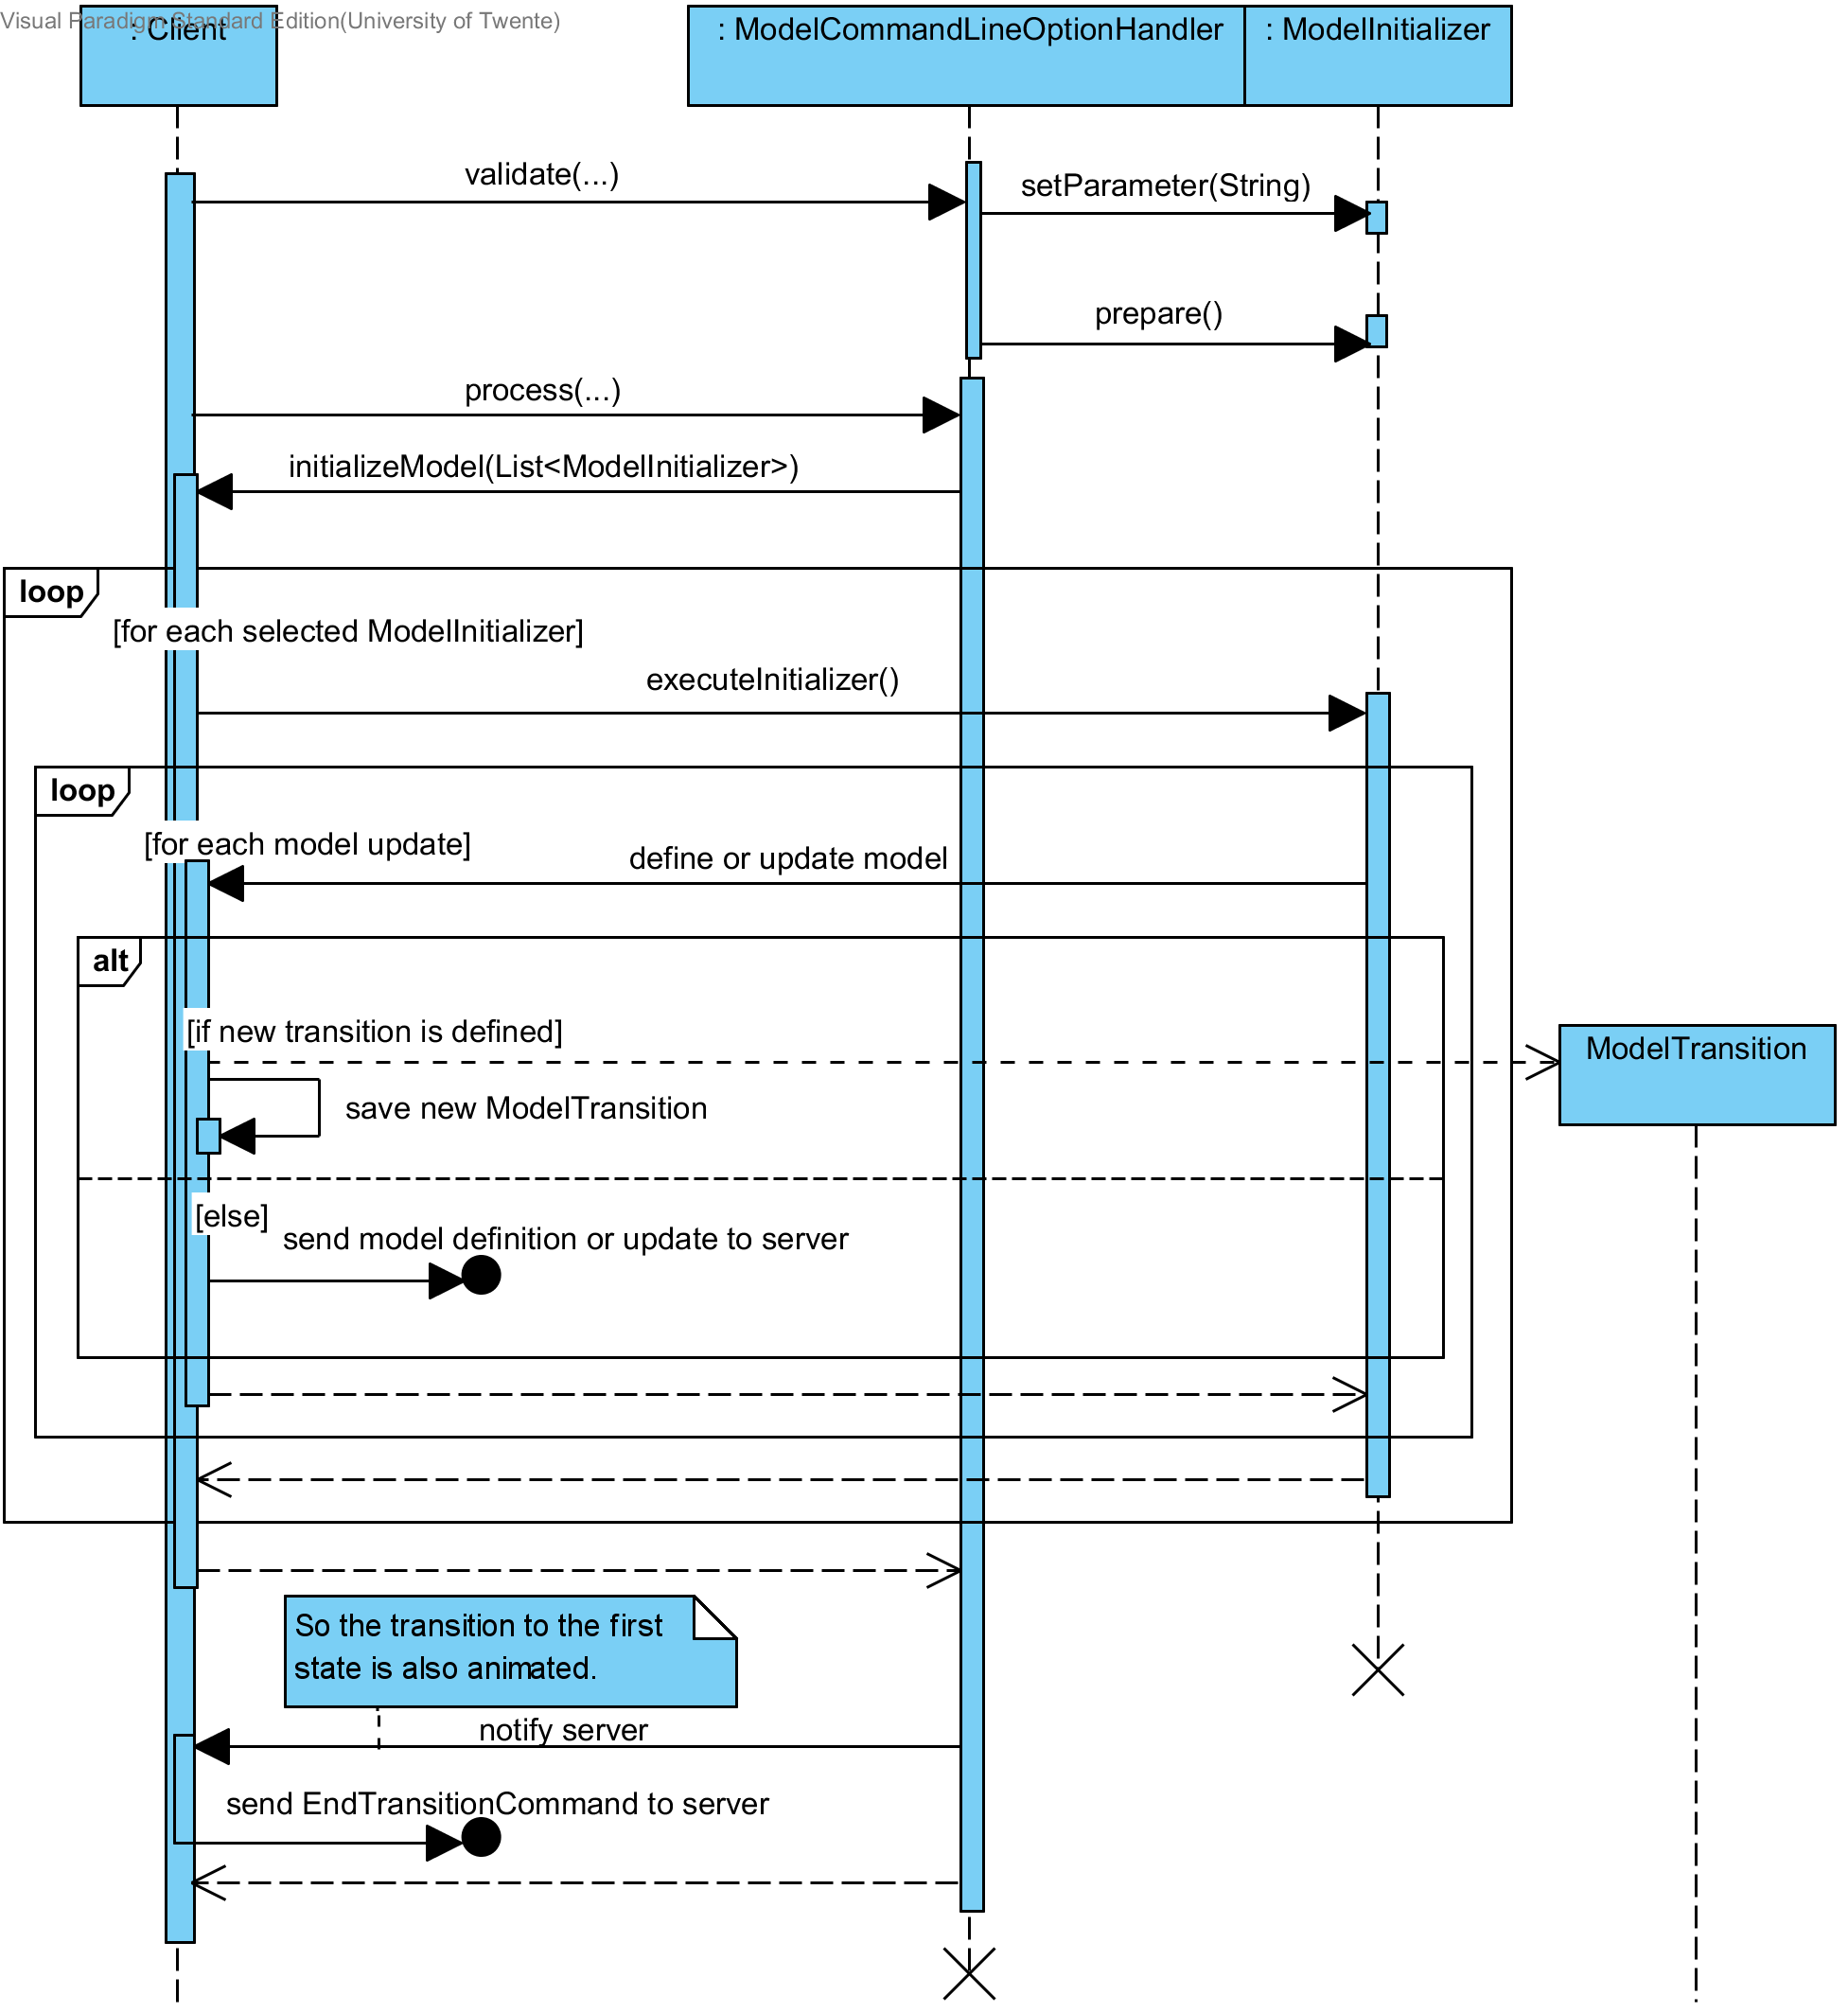
\includegraphics[width=1.1\textwidth]{diagrams/SD_client_model}
  \caption{simplified sequence diagram of the handling of the \lstinline{--model} command line option}\label{fig:sd_client_model}
\end{figure}
\begin{figure}[ht]
  \centering
  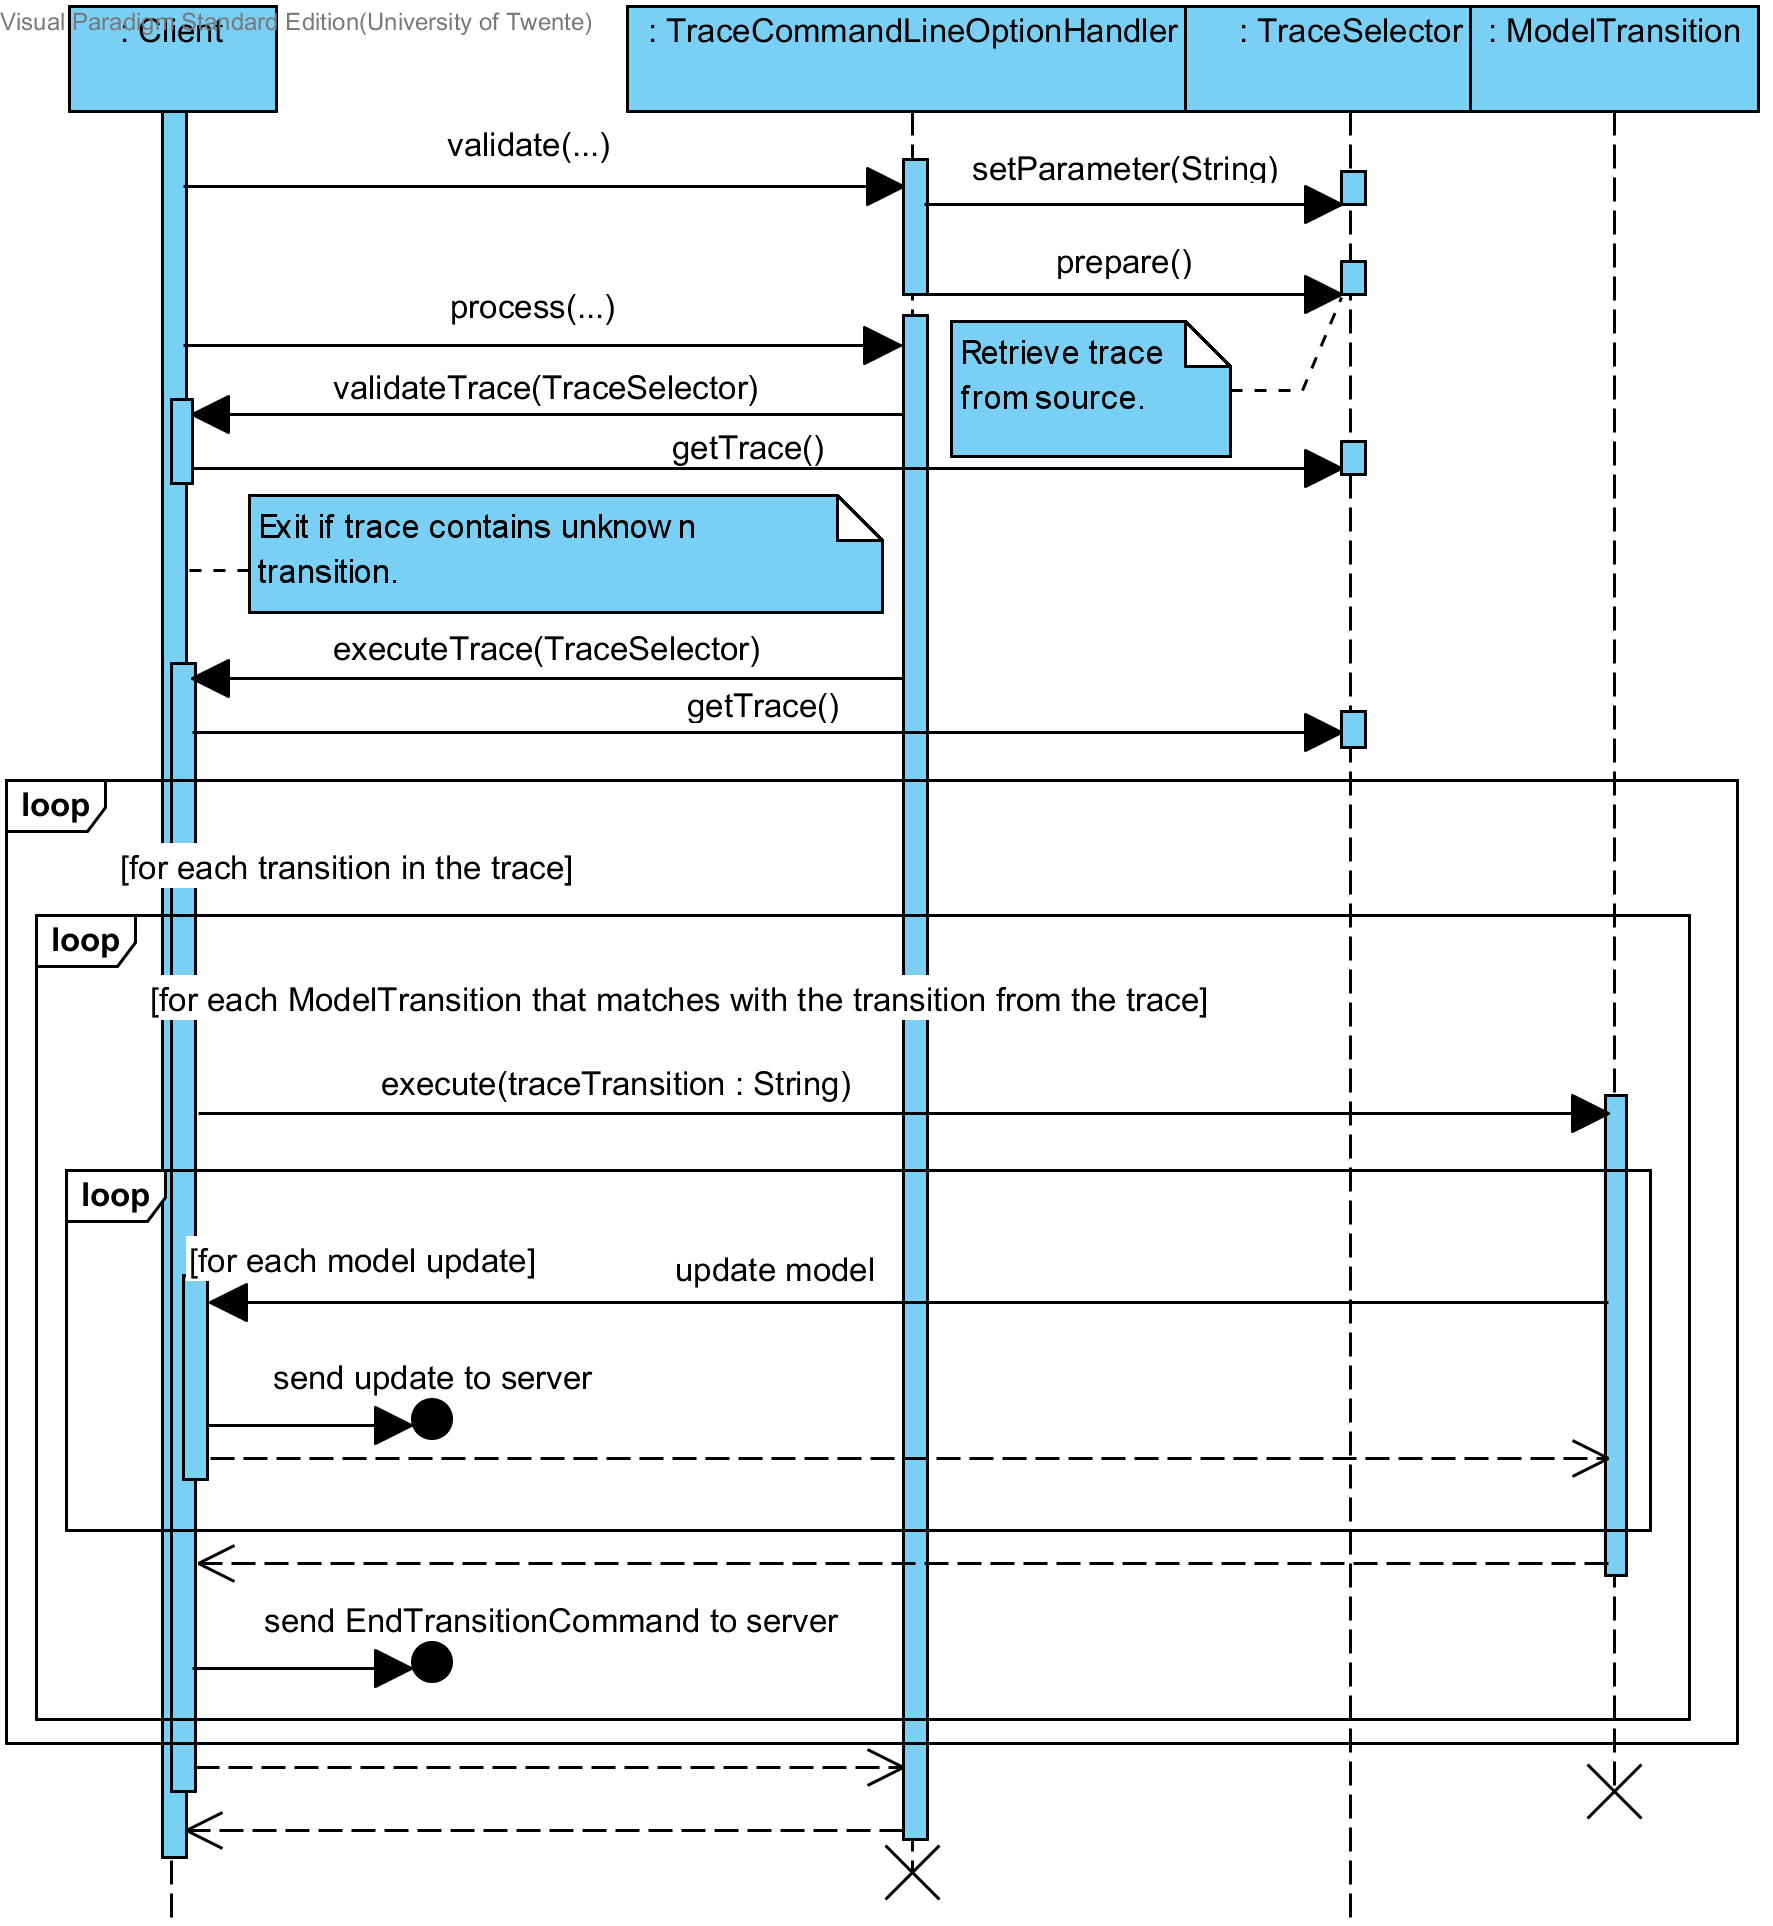
\includegraphics[width=1.1\textwidth]{diagrams/SD_client_trace}
  \caption{simplified sequence diagram of the handling of the \lstinline{--trace} command line option}\label{fig:sd_client_trace}
\end{figure}
\begin{figure}[ht]
  \centering
  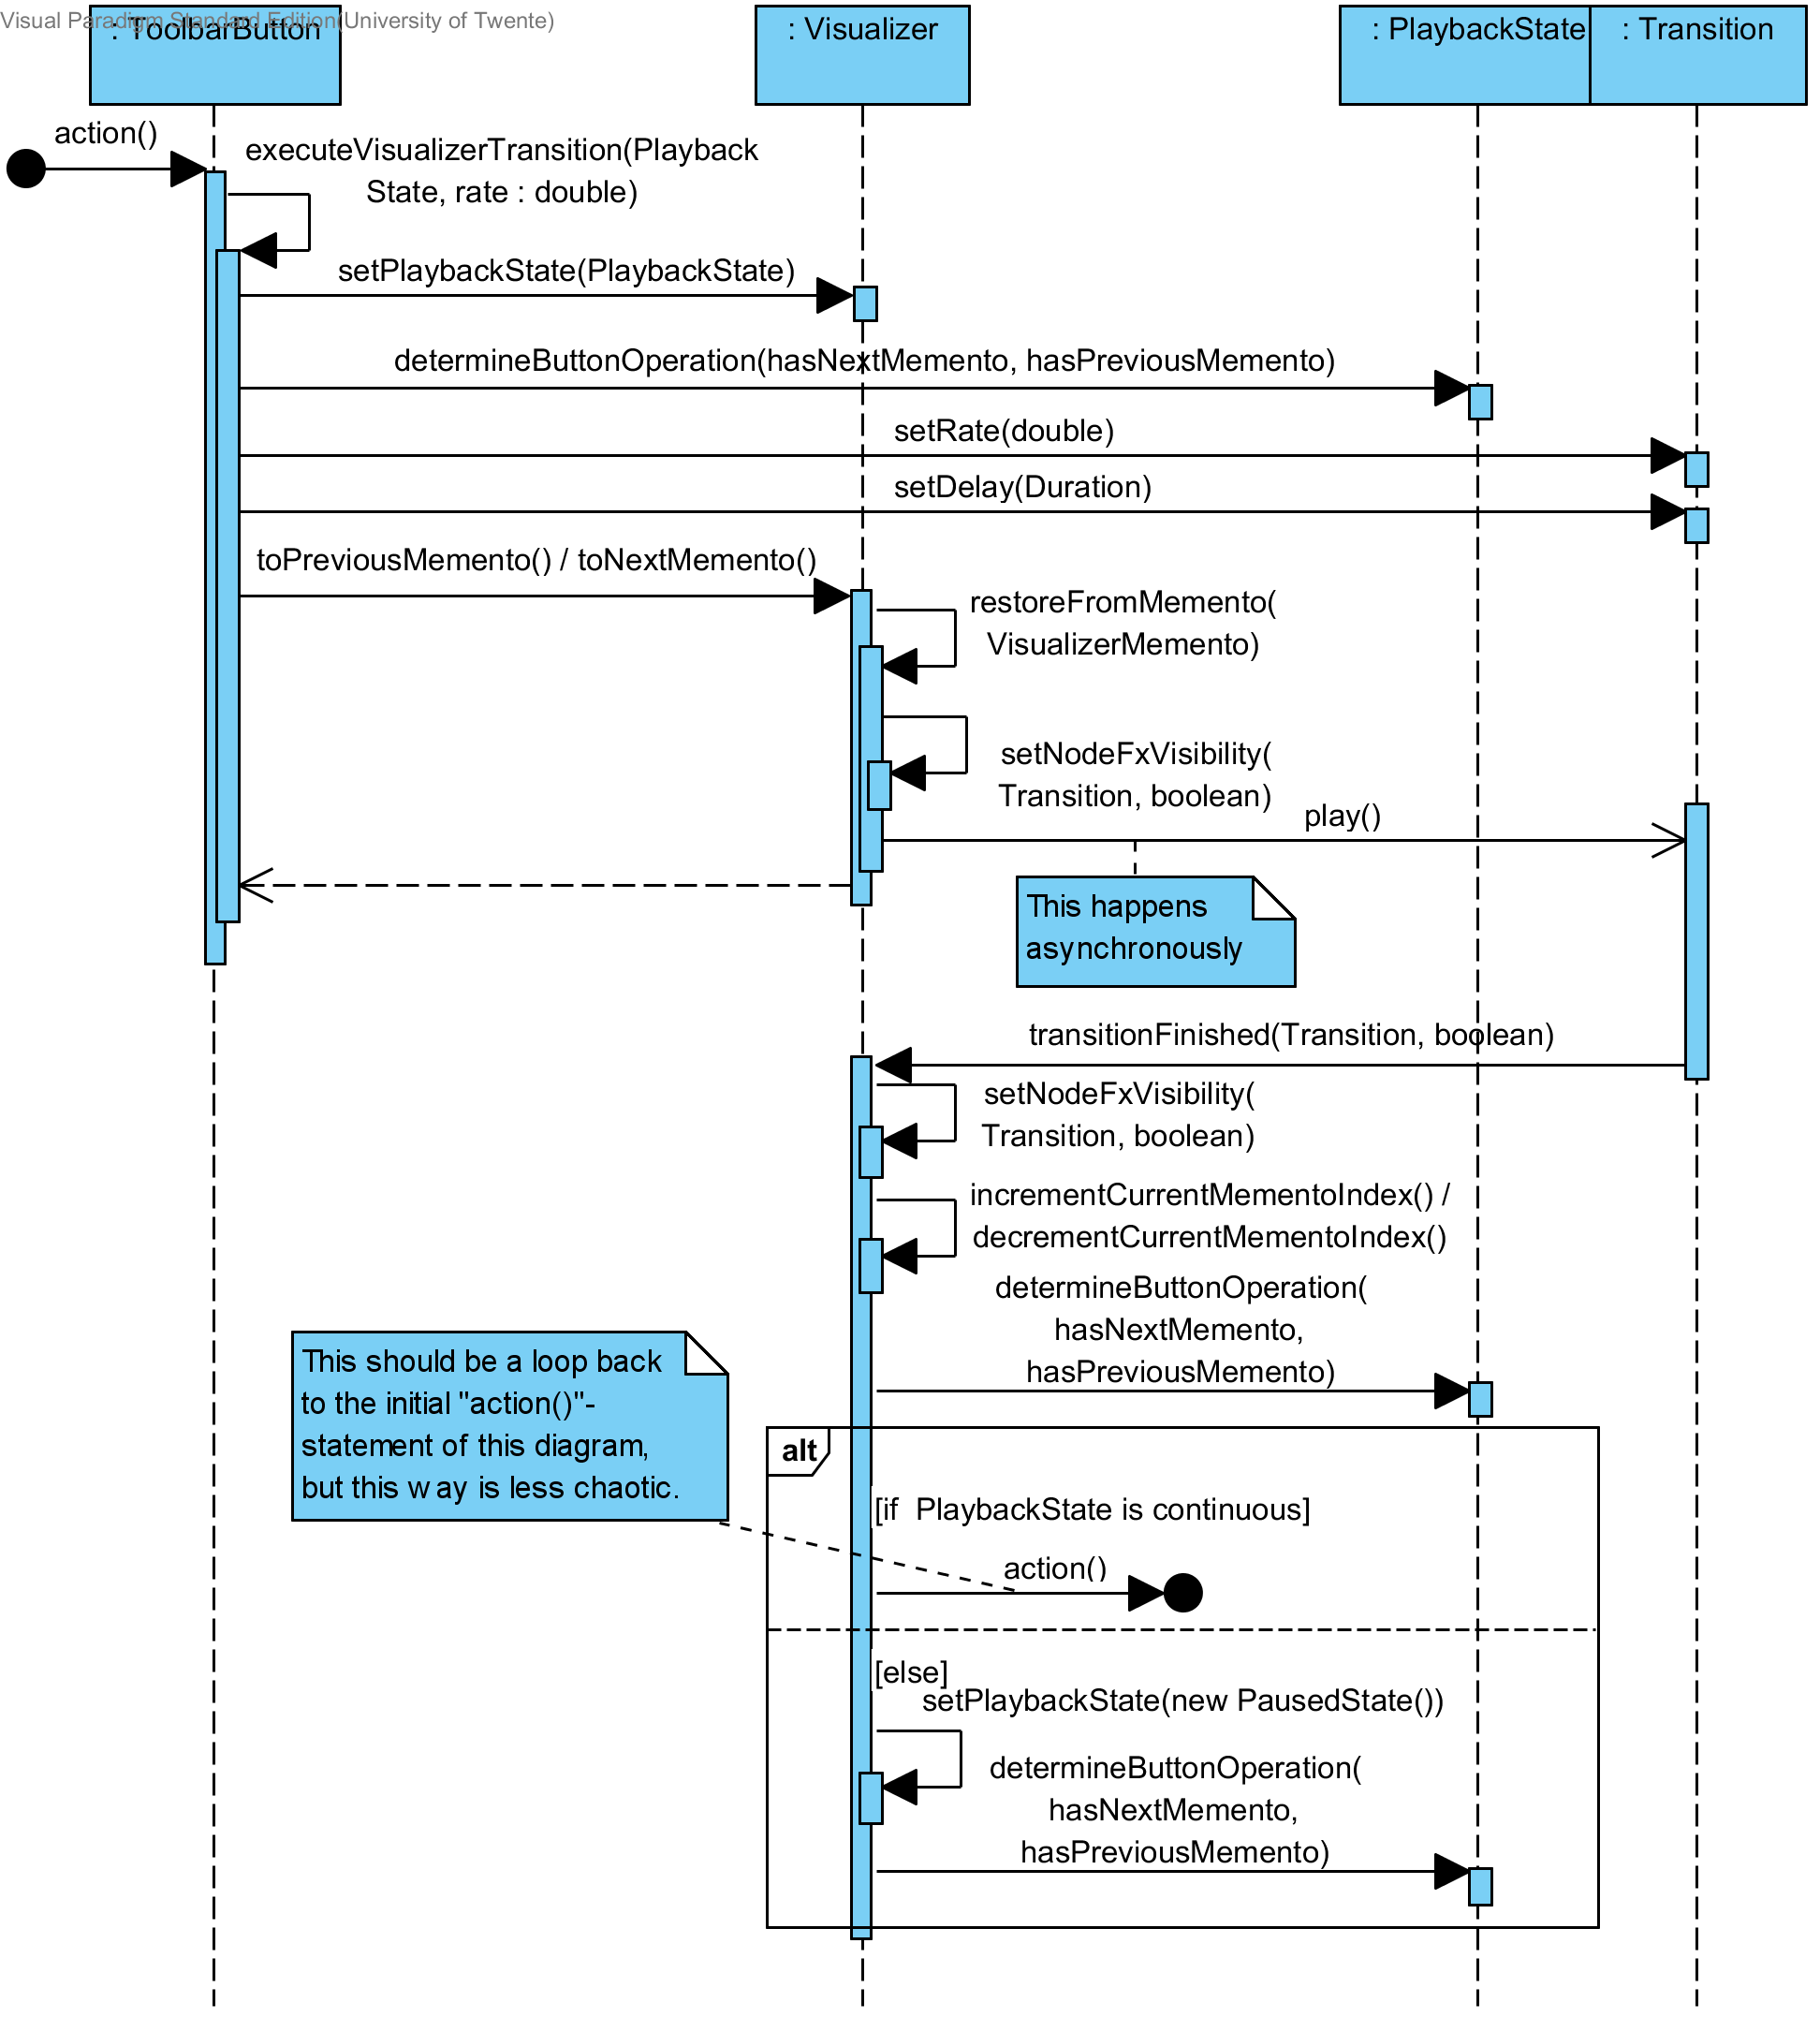
\includegraphics[width=1.1\textwidth]{diagrams/SD_server_userinteraction}
  \caption{simplified sequence diagram of user interaction with any one of the toolbar buttons (but not with the pause button)}\label{fig:sd_server_userinteraction}
\end{figure}